\documentclass[a4j,10pt,oneside,openany,fleqn]{jsbook}
%
\usepackage{amsmath,amssymb}
\usepackage{bm}
\usepackage{color}
\usepackage[dvipdfmx]{graphicx}
\usepackage{ascmac}
\usepackage{makeidx}
\usepackage{tikz}
\usetikzlibrary{matrix,calc}
%%%%


%internal group
%#1-space between node and grouping line. Default=0
%#2-top left node
%#3-bottom right node
\newcommand{\implicant}[3][0]{
  \draw[rounded corners=3pt] ($(#2.north west)+(135:#1)$) rectangle ($(#3.south east)+(-45:#1)$);
}

%group lateral borders
%#1-space between node and grouping line. Default=0
%#2-top left node
%#3-bottom right node
\newcommand{\implicantcostats}[3][0]{
  \draw[rounded corners=3pt] ($(rf.east |- #2.north)+(90:#1)$)-| ($(#2.east)+(0:#1)$) |- ($(rf.east |- #3.south)+(-90:#1)$);
  \draw[rounded corners=3pt] ($(cf.west |- #2.north)+(90:#1)$) -| ($(#3.west)+(180:#1)$) |- ($(cf.west |- #3.south)+(-90:#1)$);
}

%group top-bottom borders
%#1-space between node and grouping line. Default=0
%#2-top left node
%#3-bottom right node
\newcommand{\implicantdaltbaix}[3][0]{
  \draw[rounded corners=3pt] ($(cf.south -| #2.west)+(180:#1)$) |- ($(#2.south)+(-90:#1)$) -| ($(cf.south -| #3.east)+(0:#1)$);
  \draw[rounded corners=3pt] ($(rf.north -| #2.west)+(180:#1)$) |- ($(#3.north)+(90:#1)$) -| ($(rf.north -| #3.east)+(0:#1)$);
}

%group corners
%#1-space between node and grouping line. Default=0
\newcommand{\implicantcantons}[1][0]{
  \draw[rounded corners=3pt] ($(rf.east |- 0.south)+(-90:#1)$) -| ($(0.east |- cf.south)+(0:#1)$);
  \draw[rounded corners=3pt] ($(rf.east |- 8.north)+(90:#1)$) -| ($(8.east |- rf.north)+(0:#1)$);
  \draw[rounded corners=3pt] ($(cf.west |- 2.south)+(-90:#1)$) -| ($(2.west |- cf.south)+(180:#1)$);
  \draw[rounded corners=3pt] ($(cf.west |- 10.north)+(90:#1)$) -| ($(10.west |- rf.north)+(180:#1)$);
}

%Empty Karnaugh map 4x4
\newenvironment{Karnaugh}[2]%
               {
                 \begin{tikzpicture}[baseline=(current bounding box.north),scale=0.8]
                   \draw (0,0) grid (4,4);
                   \draw (0,4) -- node [pos=0.8,above right,anchor=south west] {#1} node [pos=0.7,below left,anchor=north east] {#2} ++(135:1);
                   %
                   \matrix (mapa) [matrix of nodes,
                     column sep={0.8cm,between origins},
                     row sep={0.8cm,between origins},
                     every node/.style={minimum size=0.3mm},
                     anchor=8.center,
                     ampersand replacement=\&] at (3.5,3.5)
                           {
                             \& |(c00)| 00         \& |(c01)| 01         \& |(c11)| 11         \& |(c10)| 10         \& |(cf)| \phantom{00} \\
                             |(r00)| 00             \& |(0)|  \phantom{0} \& |(4)|  \phantom{0} \& |(12)| \phantom{0} \& |(8)|  \phantom{0} \&                     \\
                             |(r01)| 01             \& |(1)|  \phantom{0} \& |(5)|  \phantom{0} \& |(13)| \phantom{0} \& |(9)|  \phantom{0} \&                     \\
                             |(r11)| 11             \& |(3)|  \phantom{0} \& |(7)|  \phantom{0} \& |(15)| \phantom{0} \& |(11)| \phantom{0} \&                     \\
                             |(r10)| 10             \& |(2)|  \phantom{0} \& |(6)|  \phantom{0} \& |(14)| \phantom{0} \& |(10)| \phantom{0} \&                     \\
                             |(rf) | \phantom{00}   \&                    \&                    \&                    \&                    \&                     \\
                           };
               }%
               {
                 \end{tikzpicture}
               }

               \newenvironment{Karnaughvuit}[2]%
                              {
                                \begin{tikzpicture}[baseline=(current bounding box.north),scale=0.8]
                                  \draw (0,0) grid (4,2);
                                  \draw (0,2) -- node [pos=0.7,above right,anchor=south west] {#1} node [pos=0.7,below left,anchor=north east] {#2} ++(135:1);
                                  %
                                  \matrix (mapa) [matrix of nodes,
                                    column sep={0.8cm,between origins},
                                    row sep={0.8cm,between origins},
                                    every node/.style={minimum size=0.3mm},
                                    anchor=4.center,
                                    ampersand replacement=\&] at (3.5,1.5)
                                          {
                                            \& |(c00)| 00         \& |(c01)| 01         \& |(c11)| 11         \& |(c10)| 10         \& |(cf)| \phantom{00} \\
                                            |(r00)| 0             \& |(0)|  \phantom{0} \& |(2)|  \phantom{0} \& |(6)|  \phantom{0} \& |(4)|  \phantom{0} \&                     \\
                                            |(r01)| 1             \& |(1)|  \phantom{0} \& |(3)|  \phantom{0} \& |(7)|  \phantom{0} \& |(5)|  \phantom{0} \&                     \\
                                            |(rf) | \phantom{00}  \&                    \&                    \&                    \&                    \&                     \\
                                          };
                              }%
                              {
                                \end{tikzpicture}
                              }
                              

                              %Defines  16 values (0,1,X)
                              \newcommand{\contingut}[1]{%
                                \foreach \x [count=\xi from 0] in {#1}
                                \path (\xi) node {\x};
                              }
                              

%%%
\makeindex
%
\newcommand{\diff}{\mathrm{d}}  %微分記号
\newcommand{\divergence}{\mathrm{div}\,}  %ダイバージェンス
\newcommand{\grad}{\mathrm{grad}\,}  %グラディエント
\newcommand{\xbar}[1]{\overline{x_{#1}}}
\newcommand{\rot}{\mathrm{rot}\,}  %ローテーション
%
\setlength{\textwidth}{\fullwidth}
\setlength{\textheight}{44\baselineskip}
\addtolength{\textheight}{\topskip}
\setlength{\voffset}{-0.6in}
\setcounter{chapter}{-1}
%
\title{{\Huge \textbf{計算システム論1}}\\ {\small Ver. 0.17.0}}
\author{O-green}
\date{\today}
\begin{document}

%
%
\maketitle
\frontmatter
\tableofcontents
%
%
\mainmatter

\chapter{はじめに}
\begin{abstract}
  授業の目的
  ハードウェアの設計に関する基礎理論
  VLSI上に実装する際の基本戦略
  高速 安い 信頼性
\end{abstract}

\chapter{ブール代数}

\setcounter{section}{-1}
\section{公理集}
\begin{align}
  交換律&
  \begin{cases}
    x \vee y = y \vee x
    x \cdot y = y \cdot x
  \end{cases} &\\
  結合律&
  \begin{cases}
    (x \vee y) \vee z = x \vee (y \vee z)
    (x \cdot y) \cdot Z = x \cdot (y \cdot z)
  \end{cases}&\\
  吸収律&
  \begin{cases}
    x \vee (x \cdot y) = x
    x \cdot (x \vee y) = x
  \end{cases}&\\
  分配律&
  \begin{cases}
    x \vee (y \cdot z) = (x \vee y) \cdot (x \vee z)\\
    x \cdot (y \vee z) = (x \cdot y) \vee (x \cdot y)
  \end{cases}& \\
  単位元, 零元&
  \begin{cases}
    x \vee 1 = 1
    x \cdot 0 = 0
  \end{cases}&\\
  補元律&
  \begin{cases}
    x \vee \overline{x} = 1\\
    x \cdot \overline{x} = 0
  \end{cases}& \\
  べき等律&
  \begin{cases}
    x \vee x = x
    x \cdot x = x  
  \end{cases}&  
\end{align}
\section{基本概念}
\subsection{束(Lattice)}
集合$L$上で2つの2項演算
\begin{eqnarray*}
  &&\vee : L \times L \rightarrow L \\
  &&\cdot : L \times L \rightarrow L 
\end{eqnarray*}
が定義され $L$ の任意の要素$x, y, z$に対して
(1.1),(1.2),(1.3),(1.7)の4つの公理が満たされる時この代数系 $(L, \vee, \cdot)$を\textbf{束}という。\\
束$(L, \vee, \cdot)$において(1.4)が成立するとき\textbf{分配束}という。\\
束において任意の要素が補元をもつとき\textbf{相補束}という。
補元は(1.5)で定義、単位元と零元を持つ時定義可能。
\[a \textrm{の補元が} b \Leftrightarrow a \vee b = 1, a \cdot b = 0 \]
\\
相補的かつ分配的な束を\textbf{ブール束}という。ブール束によって定義される代数系を\textbf{ブール代数}という。\\
\\
\textbf{定理} 分配束において要素が補元をもつときは補元は一意である。 $\blacksquare$

\subsection{ブール代数の定義}
\textbf{定義1.1(ブール代数)}
$B$を少なくとも2つの異なる要素0と1を含む集合とする。
$B$の上で2つの2項演算 $\vee , \cdot$ と1つの単項演算 $\overline{ }$が定義され(1.1)〜(1.6)の6つの等式(公理)を満たす時$(B, \vee, \cdot, \overline{ }, 0, 1)$ をブール代数という。

ブール代数における演算
\begin{align*}
&\vee:\textrm{論理和, OR}\\
&\cdot: \textrm{論理積, AND}&\\
&\overline{ }:\textrm{否定, NOT}&
\end{align*}
\\
$B$ の要素を値とする変数を\textbf{ブール変数} あるいは \textbf{論理変数} という。\\
ブール変数と定数に演算を0回以上適用したものを\textbf{ブール式} あるいは \textbf{論理式}という。\\
演算の優先順位は以下のとおりである\\
\[ \textrm{括弧}() > \textrm{否定}\overline{ } > \textrm{論理積}\cdot > \textrm{論理和} \vee \]

\subsection{双対性}

ある等式とその等式に対し$\vee \leftrightarrow \cdot, 0 \leftrightarrow 1$の交換をした等式は\textbf{双対(dual)}であるという。\\
双対性原理
ある等式が成立する時、その双対な等式も成立する。ただし演算の優先順位は保つ。

\section{ブール代数の基本定理と公理系}
\subsection{基本定理}
\textbf{定理1.2} ブール代数では以下が成立する。
\begin{align*}
  \textrm{(1.8)}&
  \begin{cases}
    x \vee 0 = x \\
    x \cdot 1 = x
  \end{cases}&\\
  \textrm{単位元、零元}&
  \begin{cases}
    x \vee y = 0 \Leftrightarrow x=y=0 \\
    x \cdot y = 1 \Leftrightarrow x=y=1
  \end{cases}&\\
  ド・モルガン律&
  \begin{cases}
    \overline{(x \vee y)} = \overline{x} \cdot \overline{y} \\
    \overline{(x \cdot y)} = \overline{x} \vee \overline{y}     
  \end{cases}&\\
  二重否定  &
  \overline{\overline{x}} = x&\\
  ブール吸収律&
  \begin{cases}
    x \vee (\overline(x) \cdot y) = x \vee y \\
    x \cdot(\overline(x) \vee y) = x \cdot y
  \end{cases}&  
\end{align*}

\textbf{定理(1.3)} 論理式 $F$ の否定 $\overline{F}$ は$F$ において演算の置換$(\vee \leftrightarrow \cdot)$、変数の置換 $(x_i \leftrightarrow \overline{x_i})$、定数の置換$(0\leftrightarrow 1)$を施して得られる論理式と等しい。\\

\subsection{ハンティントンの公理}

ブール代数の定理を証明するには(1.1),(1.4),(1.6),(1.8)の4つの等式で十分。


\section{順序関係の導入}

\subsubsection{順序関係}
$S_1$と$S_2$を集合とする。直積$S_1 \times  S_2$の部分集合$R$を$S_1$と$S_2$の\textbf{2項関係}という。任意の要素$s_1 \in S_1, s_2 \in S_2$に対し$(s_1, s_2) \in R$のとき$s_1$と$s_2$は関係 $R$ をもつといい、$s_1 R s_2$ と表記する。特に$S_1$ と $S_2$が同じ集合の時 $R$ を $S$ の上の2項関係という。
\\
集合$S$の上の2項関係を$R$とする。$S$の任意の要素 $x,y,z$に対して
\begin{align*}
  \begin{cases}
    \textrm{反射率: } xRx\\
    \textrm{反対称律: } xRy \wedge yRx \Rightarrow x=y \\
    \textrm{推移律: } xRy \wedge yRz \Rightarrow xRz 
  \end{cases}
\end{align*}
が成立する時 $R$ を\textbf{順序関係}、あるいは\textbf{半順序関係}という。また、$S$のすべての要素に対して $xRy$ あるいは $yRx$ が成り立つような順序関係 $R$ を全順序関係という。\\
関係 $R$ を $xRy$ と書く代わりに $x \leq y$ と書くとわかりやすいので、以下この表記を採用する。

\subsubsection{ハッセ図}
順序関係を表す図として\textbf{ハッセ図}がある。集合$S$の異なる $x,y$ に対し
\begin{align*}
  \begin{cases}
    x \leq y \textrm{であり}\\
    x \leq z \leq y \textrm{となる} z(z \neq y, x)\textrm{が存在しない}
  \end{cases}
\end{align*}
ときに$y$ を $x$ の上方に置き、両者を線で結んだものがハッセ図である。
\begin{figure}[h]
  \centering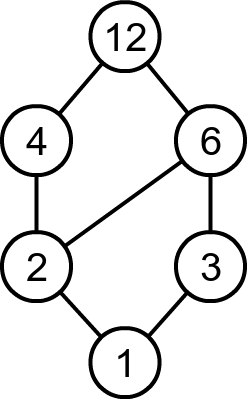
\includegraphics[height=3cm]{Images/Hasse_example.png}
  \caption{$x\leq y \Leftrightarrow$ 「$y$は$x$で割り切れる」と定義した時のハッセ図}
\end{figure}

\subsubsection{最大、極大、上界、上限}
半順序集合 $S$ のある要素 $s$に対し $s \leq a$ となる $a$ が常に $s=a$となるとき $s$を$S$の \textbf{極大元} という。\\
半順序集合 $S$ のある要素 $s$が$S$n任意の要素 $a$ に対して$a\leq s$を満たすときの $s$ を$S$の\textbf{最大限}という。\\
\textbf{極小元}や\textbf{極大元}も同様に定義される。\\
最大限や最小限はたかだか1つであり、ない場合もある。最大限(最小元)は存在するならば必ず極大元(極小元)である。\\

関係 $\leq$ が定義された半順序集合 $S$ の部分集合を $T$ とする。\\
$T$ の任意の要素 $t$ に対して $t \leq u$ が成立する $S$の要素 $u$ を $T$の\textbf{上界}という。\\
上界全体からなる集合の最小元を\textbf{上限}という。\\
\textbf{下界}、\textbf{下限}も同様に定義される。
\newpage
\subsubsection{束}
半順序集合 $(L, \leq)$においうて$L$の任意の2つの要素が必ず上限と下限をもつときその半順序集合を\textbf{束}という。

\begin{figure}[h]
  \centering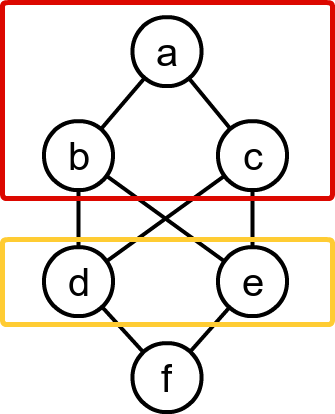
\includegraphics[height=3cm]{Images/Hasse_not_lattice.png}
  \caption{$d,e$の上界は${a,b,c}$であるが、上限は存在しない。この順序集合は束ではない。}
\end{figure}

束の順序構造としての定義と、代数的定義(1.1)は等価である。順序構造における代数的演算として
\begin{itemize}
\item $x \vee y$ を$x$と$y$の上限
\item $x \cdot y$ を $x$ と$y$の下限 
\end{itemize}
と定義すれば、(1.1)での代数的定義と矛盾しない。

\subsubsection{束における双対性}
束である順序集合 $A$ において、与えられた任意の正しい命題は、関係「$\leq$」「$\geq$」を交換、演算「$\vee$」「$\cdot$」を交換しても正しい命題となる。これらの交換は、ただ単にハッセ図を上下ひっくり返す操作に対応する。

\subsubsection{種々の束}
分配律が成立する束を \textbf{分配束}と呼ぶ。
零元と単位元が存在し、任意の要素に対し補元が存在する束を \textbf{相補束} と呼ぶ。
相補的かつ分配的な束を \textbf{ブール束}という

\chapter{論理関数の表現}

\section{論理関数と組み合わせ回路}

\subsection{論理関数}

\subsubsection{論理回路}
AND,ORなどの論理素子の相互接続で構成される回路を\textbf{論理回路}という。一般には複数の入力と複数の出力を持つ
現在の出力が現在の入力のみで決定されるような論理回路を\textbf{組み合わせ回路(combinatinaol circuit)}と呼ぶ。
それに対して、現在の出力が過去から現在までの入力の履歴に依存して決まる論理回路を\textbf{順序回路(sequential circuit)}と呼ぶ。

\subsubsection{組み合わせ回路}
出力変数は独立 $\Rightarrow$ 複数入力、1出力の組み合わせ回路が集まったものとして扱える
\\

\textbf{定義2.1(論理関数)}
$B = {0, 1}$ の上で任意の自然数 $n$ に対して定義される関数 $F:B^n \rightarrow B$ を\textbf{論理関数} という。

\subsection{真理値表と論理式}

\subsubsection{真理値表(truth table)}
\textbf{真理値表}は全通りの入力組み合わせに対して、出力の値を示す表である。
$n$ 入力の場合、 $2^n$ 個のエントリーがある。それぞれの出力が 2 通りずつあるので、$n$ 入力論理関数は $2^{2^n}$ 種類ある。
\begin{table}[htb]
  \begin{center}
    \begin{tabular}{lcr|r} 
      $x_1$ & $x_2$ & $x_3$ & $f$ \\ \hline 
      0 & 0 & 0 & 0 \\
      0 & 0 & 1 & 1 \\
      0 & 1 & 0 & 0 \\
      0 & 1 & 1 & 1 \\
      1 & 0 & 0 & 0 \\
      1 & 0 & 1 & 0 \\
      1 & 1 & 0 & 1 \\
      1 & 1 & 1 & 1 \\
    \end{tabular}
  \end{center}
  \caption{3入力真理値表の例($f = (x_1 \cdot x_2) \vee (\overline{x_1} \cdot x_3)$)}
\end{table}

\newpage

\subsubsection{論理式}
論理変数と定数に論理演算を適用して得られる式。
以下の論理式は、上の真理値表と対応する。このように論理式は真理関数に対して一意ではない
\begin{align*}
f &= \overline{x_1} \cdot \overline{x_2} \cdot x_3 \vee \overline{x_1} \cdot x_2 \cdot x_3 \vee x_1 \cdot x_2 \cdot \overline{x_3}  \vee x_1 \cdot x_2 \cdot x_3 &\\
f &= x_1 \cdot x_2 \vee \overline{x_1} \cdot x_3 \vee x_2 \cdot x_3 &\\
f &= x_1 \cdot x_2 \vee \overline{x_1} \cdot x_3 &
\end{align*}
\subsection{完全定義関数と不完全定義関数}
すべての入力組み合わせに対して出力が定義されている論理関数を\textbf{完全定義関数}と呼ぶ。
ある入力組み合わせに対して出力が定義されていない論理関数を\textbf{不完全定義関数}と呼ぶ。

\section{論理式の標準展開}
論理式の一意な表現を得るための式の展開を考える。
\subsection{極小項表現と極大項表現}

\subsubsection{積項(product term)}
1つ以上の論理変数またはその否定を論理積だけで結合した論理式を\textbf{積項}と呼ぶ。
\begin{align*}
x_1, x_1 \cdot x_2, \overline{x_1} \cdot x_2
\end{align*}
\subsubsection{積和形(sum of product)}
1つ以上の積項を論理和で結合した論理式を\textbf{積和形}と呼ぶ。
\begin{align*}
x_1 \cdot x_2 \vee \overline{x_1} \cdot x_3 \vee x_2 \cdot x_3
\end{align*}

\textbf{和項}、\textbf{和積形}も双対的に定義される。

\subsubsection{極小項}
入力変数が$n$ 個で $x_1, x_2, \dots, x_n$ で表される時、すべての $i$ に対し$x_i$ または $\overline{x_i}$ のどちらかを必ず含む積項を\textbf{極小項}と呼ぶ。

\subsubsection{極小項表現}
重複のない極小項だけを含む積和形を\textbf{極小項表現}とよぶ。


\subsubsection{極小項}
入力変数が$n$ 個で $x_1, x_2, \dots, x_n$ で表される時、すべての $i$ に対し$x_i$ または $\overline{x_i}$ のどちらかを必ず含む和項を\textbf{極大項}と呼ぶ。

\subsubsection{極小項表現}
重複のない極大項だけを含む和積形を\textbf{極大項表現}とよぶ。

\subsubsection{一意性}
任意の論理関数は極小項表現および極大項表現で一意に表せる。これらは、真理値表を書くか、式展開によって導出できる。

\subsection{ブール展開}
任意の論理関数はブール展開を繰り返し適用すると一意な積和標準系が得られる。


\textbf{定理2.1}
$F(x_1, x_2, \dots, x_n) = \overline{x_1} \cdot F(0, x_2, \dots, x_n) \vee x_1 \cdot F(1, x_2, \dots, x_n) $

\textbf{定理2.2}
$F(x_1, x_2, \dots, x_n) = (\overline{x_1} \vee F(1, x_2, \dots, x_n)) \cdot x_1 \vee F(0, x_2, \dots, x_n) $

\subsection{リード・マラー標準系}
以下の真理値表に従う論理演算子を\textbf{排他的論理和(exclusive OR)}と呼ぶ。

\begin{table}[htb]
  \begin{center}
    \begin{tabular}{cc|c} 
      $x$ & $y$ & $x\oplus y$ \\ \hline 
      0 & 0 & 0 \\
      0 & 0 & 1 \\
      0 & 1 & 1 \\
      0 & 1 & 0 \\
    \end{tabular}
  \end{center}
  \caption{排他的論理和の真理値表}
\end{table}

\textbf{定理2.3}
\begin{align*}
  (x \oplus y) \oplus z &= x \oplus ( y \oplus z)&\\
  x \oplus y &= y \oplus x&\\
  x \cdot ( y \oplus z) &= (x \cdot y) \oplus ( x \cdot z)&\\
  x \oplus 0 &=x &\\
  x \oplus x &=0&
\end{align*}

\textbf{定理2.4}
\begin{align*}
  x \vee y &= x \oplus y \oplus x \cdot y&\\
  \overline{x} &= 1 \oplus x&
\end{align*}

この定理から、いままで$\vee, \cdot, \overline{ }$ を使って表現してきた論理式は、$\oplus, \cdot$だけで表現できる。
この2つの演算子のみで表現した標準系が\textbf{リード・マラー標準系}である。\\
一般形 $f(x_1 , x_2, \cdots , x_m)$ は
\begin{align*}
  f(x_1 , x_2, \cdots , x_m) &=& \\
  & & a_0 \oplus\\
  & &a_1 \cdot x_1 \oplus a_2 \cdot x_2 \oplus \cdots \oplus a_n \cdot x_n \oplus \\
  & &a_{1,2}\cdot x_1 \cdot x_2 \oplus a_{1,3}\cdot x_1 \cdot x_3 \oplus \cdots \oplus a_{n-1,n} \cdot x_{n-1} \cdot x_n \oplus\\
  & &\vdots
\end{align*}
と書かれる。

\subsubsection{リード=マラー展開}
リード=マラー標準系は以下の\textbf{リード=マラー展開}を用いて機械的に導出できる。
\begin{align*}
  f(x_1, x_2, \cdots, x_n) &=& {x_1 \cdot (f(1, x_2, \cdots, x_n) \oplus f(0, x_2, \cdots, x_n))} \oplus f(0, x_2, \cdots, x_n)
\end{align*}

\section{BDD表現}

論理関数を2分木構造で表したものを \textbf{BDD(Binary Decision Diagram)}と呼ぶ。

\begin{figure}[h]
  \centering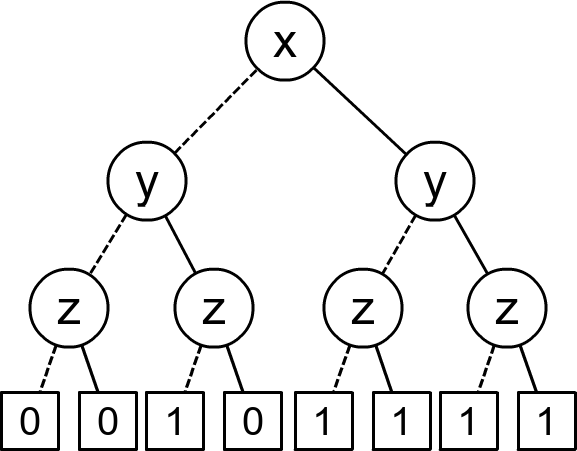
\includegraphics[height=4cm]{Images/BDD.png}
  \caption{論理式$x \vee y \cdot \overline{z}$ のBDD。根から始めて、頂点に書かれている変数の値が1なら実線、0なら破線を下向きに辿って行くと値が得られる。}
\end{figure}

論理式の変数が $n$ 個のときBDDの頂点数は $2^n$ になり膨大である。そこで、同じ部分木は一つにまとめることで頂点数を削減したものを\textbf{ROBDD(Reduced Orderd BDD)}と呼ぶ。

\begin{figure}[h]
  \centering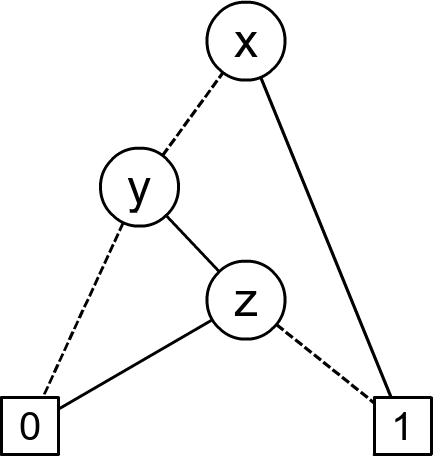
\includegraphics[height=4cm]{Images/ROBDD.png}
  \caption{論理式$x \vee y \cdot \overline{z}$ のROBDD。}
\end{figure}

変数の順番を決めればROBDDの形は一意に決まる。頂点数の最大値は $2^n$ だが、現実的なたいていのケースではもっと小さくなる。またROBDDは論理演算を再帰的に定義しているため、コンピュータで扱いやすい表現と言える。そのうえ、否定をとるのが容易である\footnote{極小(大)項表現では否定をとるとド・モルガンの公式などを使って多くの計算をしなければならなかった}。

\chapter{論理関数の性質}

\section{ユネイト関数と単調関数}

\textbf{定義3.1(包含)} 2つの$n$ 変数関数$F,G$と${0,1}^n$の任意の要素$a$ に対して $F(a) \leq G(a)$ が成立する時 $G$ は $F$を\textbf{包含する}といい$F(x) \leq G(x)$ と書く。\\
\textbf{定義3.2(関数の正負)} $F(x_1, x_2, \cdots, x_n)$ において変数 $x_i$ の値を0または1に置き換えた時 $F(x_1, \cdots, x_i, \cdots, x_n) \leq F(x_1, \cdots, x_i, \cdots, x_n)$ が成り立つ時$F$は $X$に対して\textbf{正}であるという。同様に\textbf{負}も定義できる。\\

\textbf{定理.3.1} $x_i$ に対して$F$ が正である必要十分条件は $F$ が $\overline{x}$を含まない和積形の表現を持つことである。\\

\subsubsection{ユネイト}
論理関数 $F$ がすべての変数に対して正もしくは負の時 $F$ は\textbf{ユネイト}であるという。
もし、 $F$ がすべての変数に対してせいであるならば $F$ は\textbf{正関数}であるという。

\textbf{定義3.6} 2つの$n$ 次元2値ベクトル$A = (a_1, a_2, \cdots, a_n), B = (b_1, b_2, \cdots, b_n)$が任意の $i$ に対して $a_i \leq b_i$ のとき $A \leq B$ とする。\\
\textbf{定理3.4} $n$ 変数論理関数 $F$ が正関数であるための必要十分条件は $A \leq B$ となる任意の $n$ 次元ベクトル $A,B$ に対して $F(A) \leq F(B)$ が成立するときである。\\

\section{双対関数}
\textbf{定義3.7(双対関数)}
$n$変数論理関数に対して $F_d(x_1, x_2, \cdots , x_n) = \overline{F(\overline{x_1}, \overline{x_2}, \cdots, \overline{x_n})}$をFの\textbf{双対関数(dual function)}という。

\textbf{定義3.8(自己(反)双対関数)}
$F_d(x) = F(x)$ が成立するとき$F$を自己双対関数という。
また、$F_d(x) = \overline{F_(x)}$が成立するとき $F$ を\textbf{自己反双対関数}という。

\textbf{定理3.8}
\[
G(x_1, x_2, \cdots, x_n, x_{n+1}) = x{n+1} \cdot F(x. \cdots, x_n) \vee \overline{x_{n+1}}F_d(x_1, \cdots, x_n)
\]
は自己双対関数である。

\section{その他の関数}
\subsection{対称関数}
\textbf{定義3.10(対称関数)}
$F(x_1, \cdots,x_i,\cdots, x_j, \cdots, x_n)$における任意の$x_i$と$x_j$を入れ替えて得られる関数が元の関数と等しい時 $F$ を\textbf{対称関数}という。

\textbf{例3.17}
任意の3変数対称関数は
\[
F(x,y,z) = a_0S_0 \vee a_1S_1 \vee a_2S_2 \vee a_3S_3
\]
で表せる。ただし$a_0$〜$a_3$は0または1の定数。
\begin{align*}
S_0 &= \overline{x} \cdot \overline{y} \cdot \overline{z}\textrm{ (入力の中で値が1となるものが0個の時に出力値が1となる関数)}&\\
S_1 &= x \cdot \overline{y} \cdot \overline{z} \vee \overline{x} \cdot y \cdot \overline{z} \vee \overline{x} \cdot \overline{y} \cdot z \textrm{ (入力の中で値が1となるものが0個の時に出力値が1となる関数)}&\\
S_2 &= \textrm{(入力の中で値が1となるものが2個の時に出力値が1となる関数)}\\
S_3 &= \textrm{(入力の中で値が1となるものが3個の時に出力値が1となる関数)}\\
\end{align*}

以上から $n$ 変数対称関数は$2^{n+1}$通りあることがわかる。

\subsection{しきい値関数}

\textbf{定義3.11(しきい値関数)} \\
重み(実定数)$\omega_1, \cdots, \omega_n$としきい値(実定数)$T$が存在し
\begin{align*}
  \omega_1 \cdot x_1 + \omega_2 \cdot x_2 + \cdots + \omega_n \cdots x_n \geq T \Leftarrow F(x_1, \cdots ,x_n) &= 1&\\
  \omega_1 \cdot x_1 + \omega_2 \cdot x_2 + \cdots + \omega_n \cdots x_n < T \Leftarrow F(x_1, \cdots ,x_n) &= 0&
\end{align*}
と定義される関数を\textbf{しきい値関数}という。

\textbf{定義3.12(多数決関数)}
\begin{align*}
  \omega_1 = \omega_2 = \cdots = \omega_m = 1\\
  T = k+1
  n = 2k+1
\end{align*}
のとき$F(x_1, \cdots, x_n)$を\textbf{多数決関数}という。

\textbf{定理3.11}
しきい値関数はユネイト関数である。変数 $x_i$ に着目すると
\begin{align*}
  \omega_i = 0 \rightarrow x_i\textrm{に依存しない}
  \omega_i > 0 \rightarrow x_i\textrm{に対して正}
  \omega_i < 0 \rightarrow x_i\textrm{に対して負}
\end{align*}


\subsubsection{多数決関数}
\textbf{多数決関数} $M(x, y, z) = x\cdot y\vee y\cdot z\vee z\cdot x$は自己双対関数であり、対称関数であり、単調関数である。(sugoy!)\\
$M(x,y,1) = x\vee y, M(x, y, 0) = x \cdot y$より任意の論理関数は $3$ 変数の多数決関数と否定で表現できる。

\subsection{線形関数}
\textbf{定義3.13}
リード=マラー標準系に展開した時に論理変数に関して2次以上の積項がない論理関数を\textbf{線形関数}と言う。線形関数であることと以下の形に展開できることは同値である。
\[
F(x_1, \cdots, x_n) = a_0 \oplus a_1\cdot x_1 \oplus a_2\cdot x_2 \oplus \cdots \oplus a_n \cdot x_n
\]

\textbf{定理3.14}
$n$ 変数の線形関数は $2^{n+1}$

\textbf{定理3.16}
線形関数は自己双対関数または自己反双対関数である。

\textbf{定義3.14(ブール微分)}\\
$n$ 変数論理関数 $F(x_1, \cdots, x_i,\cdots ,x_n) (1 \leq i \leq n)$に対して
\[
\frac{\partial F}{\partial x_i} := F(x_1,\cdots, 0, \cdots, x_n) \oplus F(x_1,\cdots, 1, \cdots, x_n)
\]
を$F$の $x_i$ に関する\textbf{ブール微分} という。\\
論理関数$F$の$x_i$に関するブール微分が恒等的に0のとき$F$ は $x_i$ に依存せず、恒等的に1のとき$F$ は $x_i$ の値が変わると必ず変化する。

\textbf{定理 3.17}
論理関数$F(x_1, \cdots, x_n)$が線形関数であるための必要十分条件は、すべての変数 $x_i$に関して
\[
\frac{\partial F}{\partial x_i} = a_i (\textrm{0または1})
\]
が成立することである。


\subsubsection{故障検出}
$n$変数論理関数でモデル化できるシステム(例えば電子回路)で故障が起きたとき、いずれかの入力変数が 0 または 1に固定される\textbf{縮退故障}である場合がある。
もし$x_i$ が0に縮退しているかどうか調べたければ、 $F(x_i = 0) \oplus F(x_1, \cdots, x_n) = 1$となる $x_1, \cdots, x_n$を見つければ良い。
これは $x_i = 1$かつ $\frac{\partial F}{\partial x_i} = 1$を満たすような $x_1, \cdots, x_n$と同値である。

\chapter{論理合成}
与えられた論理関数を高性能かつ低コストな、つまり最小のゲート数で実現する論理回路を合成したい。どこまでゲート数が小さくなるかは論理素子の種類による。

\section{AND-OR 2段形式}
\begin{itemize}
\item 積和系の論理式に対応した2段の論理回路である。
\item ANDゲートとORゲートで論理を合成することに相当
\item NANDゲートのみを用いた場合にも適用可(NANDはユニバーサル)
\end{itemize}

\subsubsection{論理合成の課題}
\begin{itemize}
\item 積項の数を最小化(2段目のANDの最小化)
\item 各積項に含まれる、変数の数の最小化(1段目のORの最小化)
\end{itemize}

\section{カルノー図による論理式簡単化}
\subsubsection{カルノー図 Karnaugh map}
\textbf{カルノー図(Karnaugh map)}は真理値表を図で表現したものである。変数が5つを超えると紙には書けなくなる。

\begin{center}
  \begin{figure}[h]
    \centering
    \begin{Karnaugh}{$\tt{x_1 x_2}$}{$\tt{x_3 x_4}$}
      \contingut{0,0,1,1,1,0,0,0,0,0,1,1,0,0,0,1}
      \implicant{4}{4}
      \implicant{15}{11}
      \implicantcostats[3pt]{3}{10}
      
    \end{Karnaugh}
    \caption{$f=\overline{x_1}\cdot x_2 \cdot \overline{x_3}\cdot \overline{x_4} \vee x_1 \cdot x_3 \cdot x_4 \vee \overline{x_2}\cdot x_3$に対応するカルノー図。囲われている範囲が含意項と対応する。}
  \end{figure}
\end{center}

\subsubsection{含意項と主項}
\textbf{定義4.1}
論理関数$f$と論理積$p$に対して$p\leq f$が成り立つならば$p$を$f$の\textbf{含意項(implicant)}という。

\textbf{定義4.2}
論理関数$f$の含意項$p$に関して$p$を構成する変数のどの1つを除いても、もはや$f$の含意項にならないならば$p$を$f$の\textbf{主項(prime implicant)}という。主項はカルノー図において1のみが含まれる矩形区間に対応する。

\textbf{定理4.1}
論理関数$f$の最小積和形論理式は$f$の主項のみの和で表される。\footnote{必ずしも主項すべてを使う必要はないことに注意。}

\subsubsection{ドントケア(出力が定義されない入力がある場合)}

ドントケアがある場合、主項を求めるときは$\ast$を1とみなし、必須主項を求めるときは$\ast$を0とみなして、通常と同様のカルノー図を書けば良い。

\begin{figure}[h]
  \begin{center}
    \begin{tabular} {c}
      \begin{minipage}{0.33\hsize}
      \centering
      \begin{Karnaugh}{$\tt{x_1 x_2}$}{$\tt{x_3 x_4}$}
        \contingut{1,0,0,0,1,1,1,0,1,1,$\ast$,$\ast$,$\ast$,$\ast$,$\ast$,$\ast$}        
      \end{Karnaugh}
      \caption{ドントケアがある場合のカルノー図。7segLEDの左上の点灯と対応する。}
      \end{minipage}
      
      \begin{minipage}{0.33\hsize}
        \centering
      \begin{Karnaugh}{$\tt{x_1 x_2}$}{$\tt{x_3 x_4}$}
        \contingut{1,0,0,0,1,1,1,0,1,1,1,1,1,1,1,1}
        \implicant[2pt]{12}{10}
        \implicant{0}{8}
        \implicant[3pt]{4}{13}
        \implicantdaltbaix[4pt]{4}{14}
        
      \end{Karnaugh}
      \caption{主項を求めるときのカルノー図。これから、$f=\overline{x_3}\overline{x_4} \vee x_2 \overline{x_3} \vee x_2 \overline{x_4} \vee x_1$と表せる。}
    \end{minipage}
      
      \begin{minipage}{0.33\hsize}
        \centering
      \begin{Karnaugh}{$\tt{x_1 x_2}$}{$\tt{x_3 x_4}$}
        \contingut{1,0,0,0,1,1,1,0,1,1,0,0,0,0,0,0}
        \implicant{0}{4}
        \implicant[3pt]{4}{5}
        \implicant{8}{9}
        \implicantdaltbaix[4pt]{4}{6}

        
      \end{Karnaugh}
      \caption{必須主項を求めるときのカルノー図。$f=\overline{x_1}\overline{x_3}\overline{x_4} \vee \overline{x_1}x_2\overline{x_3} \vee x_1\overline{x_2}\overline{x_3} \vee \overline{x_1}x_2\overline{x_4}$と表せる。}
      \end{minipage}
    \end{tabular}
  \end{center}
\end{figure}




\subsection{クワイン・マクラスキー法}
\textbf{クワイン・マクラスキー法}はカルノー図と同じ手順を用いて、最小積和形論理式を求めるアルゴリズムである。
\subsubsection{手順}
\begin{description}
\item [(STEP1)] すべての主項を生成。
\item [(STEP2)] すべての極小項を覆うのに必要な最小の主項の集合を見つける。
\end{description}

\subsubsection{(STEP1)の再帰的手続き}
\begin{description}
  \item [手順1]$f=1$またはドントケアとなるすべての極小項の集合を求め、これを1次集合とする。肯定変数の数で分割し、手順2へ進む
  \item [手順$k(k>1$)]第$k-1$次集合に対して $xP\vee\overline{x}P=P$の簡単化。得られた新しい分割を第 $k$ 次集合とする。もし$k-1$次集合と$k$次集合が異なるならば、手順$k+1$に進む。そうでないなら$k$次集合が関数$f$のすべての主項からなる集合である。
\end{description}

\subsubsection{(STEP2)の詳細}
$f=1$となるすべての極小項の集合を$S$とする。STEP1で得た主項との包含関係を記す。そこに、以下の規則を適用し最小被覆集合を求める。\footnote{これらの規則に適用順序の決まりはない。順序によって得られる最小被覆集合が異なることがある。また場合によっては最小被覆集合が求まらない場合もある。そのときは分枝限定法を使うことで決定できる。}
\begin{description}
\item [規則1]$S$に含まれるある極小項を覆う主項がちょうど1つだけある場合、その主項は必須主項である。その主項が覆う極小項を$S$から除いてSTEP2を継続。
\item [規則2]ある主項$A$が覆う極小項集合 を 別の主項 $B$ が覆う極小項集合に完全に含まれていたら、主項$A$を削除してSTEP2を継続する。
\item [規則3]ある極小項集合 $C$ を覆うすべての主項が別の極小項 $D$ を覆うとき、$S$ から$D$を削除。
\end{description}



\subsubsection{STEP1具体例}
\begin{table}[htb]
  \begin{center}
    \begin{tabular}{lcr|r} 
      $x_1$ & $x_2$ & $x_3$ & $f$ \\ \hline 
      0 & 0 & 0 & $\ast$ \\
      0 & 0 & 1 & 1 \\
      0 & 1 & 0 & 0 \\
      0 & 1 & 1 & 1 \\
      1 & 0 & 0 & 0 \\
      1 & 0 & 1 & $\ast$ \\
      1 & 1 & 0 & 1 \\
      1 & 1 & 1 & 0 \\
    \end{tabular}
  \end{center}
\end{table}

\textbf{手順1}
以下の極小項の集合が1次集合になる。肯定変数の個数で昇順に並べている。
\begin{align*}
  \{\xbar{1}\xbar{2}\xbar{3}, \xbar{1}\xbar{2}x_3, \xbar{1}x_2 x_3, x_1 \xbar{2} x_3, x_1 x_2 \xbar{3}\}
\end{align*}

\textbf{手順2}
肯定変数の個数が1つだけ異なる2つについて、$xP \vee \overline{x}P = P$の簡単化ができないか試行する。
\begin{align*}
  \{\xbar{1}\xbar{2}, \xbar{1} x_3, \xbar{2} x_3, x_1 x_2 \xbar{3}\}
\end{align*}

\textbf{手順3}
もうこれ以上簡単化できない。得られた集合が主項の集合である。



\chapter{順序回路}
\textbf{順序回路(sequential circuit)}は、入力履歴を内部状態として記憶する論理回路である。
\section{オートマトン順序回路}
\textbf{オートマトン(automaton)}はギリシャ語で自動機械の意である。計算機科学の文脈では以下のような性質のうちいくつかを満たすシステムの抽象モデルを指す。
\begin{enumerate}
  \item 外部からの情報を保持する。
  \item 内部に状態を保持する。
  \item 外部へ情報を出力する。
  \item 外部からの入力と現在の内部状態で次の内部状態が決まる。
  \item 外部からの入力と現在の内部状態で外部への出力が決まる。
\end{enumerate}
一般的には1,2,4の性質を満たすものをオートマトンと言う。
有限状態\footnote{有限種類の内部状態しかとらないことを意味する。}のオートマトンは
\begin{align*}
  &M = (K, \Sigma, \delta, q_0, F)\\
  &K:\textrm{状態集合}\\
  &\Sigma:\textrm{状態集合}\\
  &\delta:\textrm{状態集合}\\
  &q_0:\textrm{初期状態}\\
  &F:\textrm{最終状態集合}
\end{align*}
と表される。

\subsubsection{出力付きのオートマトン}
我々の興味は、一般のオートマトンに加えて3,5の性質を満たす\textbf{出力付きのオートマトン}にある。

\section{順序回路の実現}
\subsection{形式定義}
\subsubsection{ミーリー型(Mealy-type)}
以下の5項の組で定義される。
\begin{align*}
  &M = (X, Q, Z, \delta, \omega)\\
  &X:\textrm{入力の集合}\\
  &Q:\textrm{状態の集合}\\
  &Z:\textrm{出力の集合}\\
  &\delta:X \times Q \rightarrow Q\textrm{なる状態遷移関数}\\
  &\omega:X \times Q \rightarrow Z\textrm{なる出力関数}
\end{align*}


\subsubsection{ムーア(Moore-type)}
以下の5項の組で定義される。ミーリー型との差異は$\omega$のみである。
\begin{align*}
  &M = (X, Q, Z, \delta, \omega)\\
  &X:\textrm{入力の集合}\\
  &Q:\textrm{状態の集合}\\
  &Z:\textrm{出力の集合}\\
  &\delta:X \times Q \rightarrow Q\textrm{なる状態遷移関数}\\
  &\omega:Q \rightarrow Z\textrm{なる出力関数}
\end{align*}

\section{フリップフロップ}
\textbf{記憶素子(フリップフロップ)}は2つの内部状態を持つ記憶素子である。与えられた論理関数を実現する順序回路を作る場合、採用する記憶素子の動作に依存してその設計は変わってくる。

\subsubsection{(ラッチ(非同期式フリップフロップ)}
\textbf{ラッチ(Latch)}は2入力 $(S, R)$ 、2出力 $(Q, \overline{Q})$型のフリップフロップである。
以下の性質を満たす
\begin{itemize}
  \item $S=R=0$: $Q, \overline{Q}$は値を維持。状態を保つ。
  \item $S=1, R=0$: $Q = 1, \overline{Q} = 0$。状態をSetする。
  \item $S=0, R=1$: $Q = 0, \overline{Q} = 1$。状態Resetする。
  \item $S=R=1$: 禁止入力。
\end{itemize}
\begin{figure}[h]
  \centering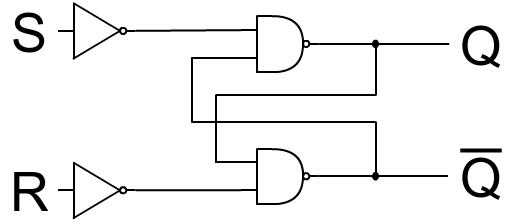
\includegraphics[height=3cm]{Images/Latch.png}
  \caption{ラッチを実現する回路}
\end{figure}


\subsubsection{フリップフロップ(同期式フリップフロップ)}
\textbf{フリップフロップ}はクロック信号に同期して状態が変化する記憶素子である。状態遷移はクロック毎に発生する。

\subsubsection{(1)SRフリップフロップ}
入力信号が安定しているときに十分幅の短いクロックが入力されるという仮定のもとで、以下のような入力駆動条件を持つフリップフロップ回路である。
\begin{table}[htb]
  \begin{center}
    \begin{tabular}{cc|cc} 
      $Q_t$ & $Q_{t+1}$ & $S$ & $R$ \\ \hline 
      0 & 0 & 0 & $\ast$ \\
      0 & 1 & 1 & 0 \\
      1 & 0 & 0 & 1 \\
      1 & 1 & $\ast$ & 0 \\
    \end{tabular}
  \end{center}
  \caption{SRフリップフロップの入力駆動条件}
\end{table}
\begin{figure}[h]
  \centering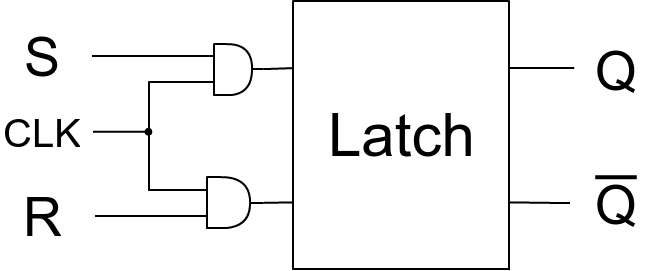
\includegraphics[height=3cm]{Images/Flipflop.png}
  \caption{SRフリップフロップ実現する回路}
\end{figure}


\subsubsection{(2)Dフリップフロップ}
\textbf{Dフリップフロップ}はクロック入力とD入力からなるフリップフロップである。
動作として、Dの入力が1なら次の状態は1であり、Dの入力が0ならば次の入力が0になる。
\begin{table}[htb]
  \begin{center}
    \begin{tabular}{cc|cc} 
      $Q_t$ & $Q_{t+1}$ & $D$  \\ \hline 
      0 & 0 & 0 \\
      0 & 1 & 1 \\
      1 & 0 & 0 \\
      1 & 1 & 1 \\
    \end{tabular}
  \end{center}
  \caption{Dフリップフロップの入力駆動条件}
\end{table}

\begin{figure}[h]
  \centering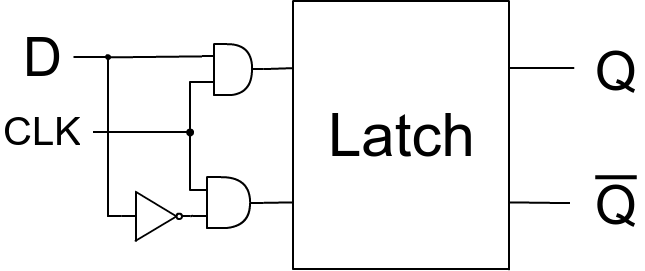
\includegraphics[height=3cm]{Images/DFlipflop.png}
  \caption{Dフリップフロップ実現する回路}
\end{figure}

\subsubsection{(3)Tフリップフロップ}
そういうのがある

\subsubsection{(4)JKフリップフロップ}
\textbf{JKフリップフロップ}はクロック入力とJ入力とK入力からなるフリップフロップである。
入力駆動条件はSRフリップフロップとほぼ同じだが、$J=K=1$となる入力が新たに許可されている。
$J=K=1$の場合状態を反転するようになっている。
\begin{table}[htb]
  \begin{center}
    \begin{tabular}{cc|cc} 
      $Q_t$ & $Q_{t+1}$ & $J$ & $K$ \\ \hline 
      0 & 0 & 0 & $\ast$ \\
      0 & 1 & 1 & $\ast$ \\
      1 & 0 & $\ast$ & 1 \\
      1 & 1 & $\ast$ & 0 \\
    \end{tabular}
  \end{center}
  \caption{SRフリップフロップの入力駆動条件}
\end{table}


\subsubsection{マスタースレーブ方式フリップフロップ}
今までの回路では「入力が安定時に十分幅の短いクロックが入る」という仮定がされていた。
これはフリップフロップの出力が安定する前に入力が変化すると誤動作する可能性があるという\textbf{タイミング問題}のためである。
\textbf{マスタースレーブ方式フリップフロップ}はその仮定が成立しない時ででもうまく動作する。
マスタースレーブ方式のフリップフロップは、マスターフリップフロップとスレーブフリップフロップの2つで構成される。
スレーブのクロック入力はマスターのクロック入力の反転を与える。


\begin{figure}[h]
  \centering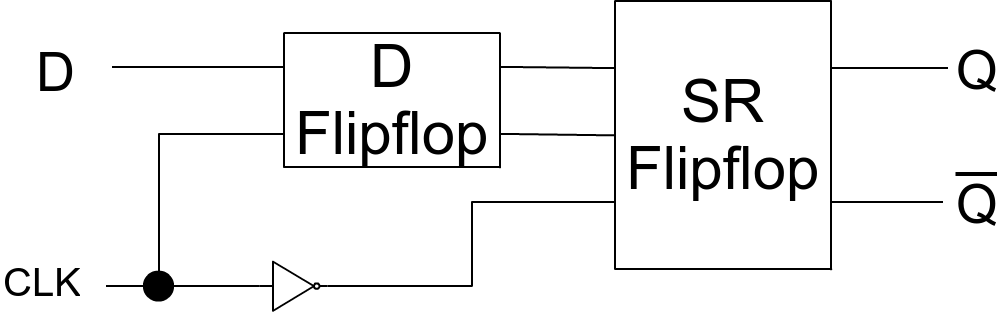
\includegraphics[height=3cm]{Images/DMasterSlave.png}
  \caption{マスタースレーブ方式のDフリップフロップ。Dフリップフロップをマスターとし、SRフリップフロップをスレーブとしている。}
\end{figure}

\subsubsection{エッジトリガ方式フリップフロップ}
\textbf{エッジトリガ方式フリップフロップ(Edge-Trigger)}はクロック信号の立ち上がり時点の入力のみで次の状態を決定するフリップフロップである。
エッジトリガ方式フリップフロップを実現する回路図は複雑である。

\subsection{順序回路の合成}
与えられた動作仕様から順序回路を導出することを考えたい。以下のようなプロセスで導出することができる。

\begin{enumerate}
\item[(1)]動作仕様を状態遷移図などの形式的記述で与える。
\item[(2)]状態遷移図を簡単化する。
\item[(3)]使用するフリップフロップの種類と数を決定する。
\item[(4)]入力駆動条件を用いて状態遷移関数と出力関数を導出。
  
\end{enumerate}

\begin{thebibliography}{20}
\bibitem{...}...
  ...
\end{thebibliography}

\newpage
\printindex
%
%
\end{document}
